\documentclass[../main/main.tex]{subfiles}

\raggedbottom

\makeatletter
\renewcommand{\@chapapp}{\'Electrocin\'etique -- chapitre}
\makeatother

\begin{document}
\setcounter{chapter}{3}

\chapter{Oscillateurs harmonique et amorti}

Dans le chapitre précédent, nous avons vu des systèmes qui présentent un régime
transitoire caractérisé par des exponentielles croissantes ou décroissantes. En
combinant deux de ces composants, on trouve alors des régimes transitoires
caractérisé par une combinaison d'exponentielles, exprimée sous la forme de
fonctions sinusoïdales. Regardons un exemple.

\section{Introduction harmonique}

\subsection{Signal sinusoïdal}

\begin{tcbraster}[raster columns=2, raster equal height=rows]
    \begin{defi}[label=def:signsu]{signal sinusoïdal}

        Un signal sinusoïdal est un signal de la forme
        \[ \boxed{s(t) = A\cos(\wt + \f)}\]

        $A$ est l'\textit{amplitude}, telle que
        \[ A = \frac{s_{\max} - s_{\min}}{2}\]

        $\wt +f$ est la \textit{phase instantanée} du signal, avec
        \vspace*{-20pt}
        \begin{center}
            \begin{tikzpicture}[]
                \node[anchor=center] (name) at (0,0)
                    {\textcolor{cornflowerblue}{$\w$}$t$+\textcolor{limegreen}{$\f$}};
                \node[inner sep=0] (datab) at ([shift={(0,3pt)}]name.south west) {};
                \node[inner sep=0] (biasb) at ([shift={(0,3pt)}]name.south east) {};
                \node[below left =.5cm and .5cm of datab, color=cornflowerblue] (data)
                    {pulsation};
                \node[below right=.5cm and .5cm of biasb, color=limegreen] (bias)
                    {phase initiale};
                \draw[-stealth] (data) -- (datab);
                \draw[-stealth] (bias) -- (biasb);
            \end{tikzpicture}
        \end{center}
        \tcbsubtitle[before skip=\baselineskip,
        colback=green!50!black,
        colframe=green!50!black]{Unités}
        La phase s'exprime en \textbf{radians}~; la pulsation en
        \textbf{\si{rad.s^{-1}}}.
    \end{defi}
    \begin{exem}[label=exem:graph]{graphique}
        \begin{center}
            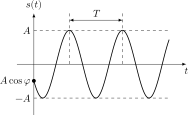
\includegraphics[width=\linewidth]{ch8-fig1}
        \end{center}
        La pulsation représente la vitesse avec de variation de la phase, et
        s'exprime en \si{rad.s^{-1}}. Pour une variation de $2\pi$ effectuée à
        la période $T$, on définit
        \begin{center}
            \fbox{$\w = 2\pi/T = 2\pi f$}
        \end{center}
    \end{exem}
\end{tcbraster}

\subsection{Équation différentielle oscillateur harmonique}

\begin{tcbraster}[raster columns=2, raster equal height=rows]
    \begin{prop}[label=prop:eqdiffoh]{équation différentielle}
        Un oscillateur harmonique à un degré de liberté est un système dont
        l'évolution temporelle est décrite par une grandeur $x(t)$ solution
        d’une équation différentielle du type~:

        \[ \boxed{ \dv[2]{x}{t} + \w_0{}^2x = \w_0{}^2x_{\rm eq}}\]

        Avec $x_{\rm eq}$ la position d'équilibre du système et $\w_0$ la
        pulsation \textbf{propre}.
    \end{prop}
    \begin{prop}[label=prop:soluoh]{solutions}
        La forme générale des solutions d'un oscillateur harmonique s'écrit de
        manière équivalente
        \begin{empheq}[box=\fbox]{gather*}
            x(t) = A'\cos(\w_0 t + \f) + x_{\rm eq}\\
            x(t) = A\cos(\w_0 t) + B\cos(\w_0 t) + x_{\rm eq}
        \end{empheq}
        avec $A'$, $A$, $B$ des \textit{constantes d'intégration}.
    \end{prop}
\end{tcbraster}

\subsection{Changement de variable~: de général à homogène}
\begin{tcbraster}[raster columns=2, raster equal height=rows]
    \begin{rema}[label=demo:chvar]{changement de variable}
        Au cours du chapitre précédent, nous avons vu la méthode pour résoudre
        des équations différentielles du premier ordre. Nous avons pu remarquer
        que les équations différentielles entre les échelons montants et
        descendants étaient en tout point similaire si ce n'est pour la présence
        ou non d'un second membre, impliquant la recherche d'une solution
        particulière ou non. Le changement de variable permet d'éviter de
        chercher une solution particulière constante.
    \end{rema}
    \begin{prop}[label=prop:chvar]{changement de variable}
        Si $x(t)$ est solution de
        \[ \boxed{ \dv[2]{x}{t} + \w_0{}^2x = \w_0{}^2x_{\rm eq}}\]
        alors $y(t) = x(t) - x_{\rm eq}$ est solution de
        \[ \boxed{ \dv[2]{y}{t} + \w_0{}^2y = 0}\]
    \end{prop}
\end{tcbraster}

\subsection{Exemple expérimental~: l'oscillateur LC}

Soit le circuit suivant sous un échelon de tension descendant. On observe la
tension $u_C(t)$ avec un oscilloscope dont la courbe est représentée à droite.

\begin{minipage}{0.50\linewidth}
    \begin{center}
        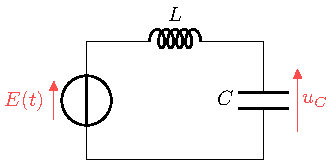
\includegraphics[width=\linewidth]{lc_descendant}
    \end{center}
\end{minipage}
\begin{minipage}{0.50\linewidth}
    \begin{center}
        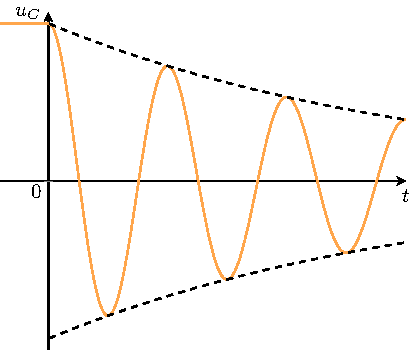
\includegraphics[width=.7\linewidth]{carac-lc_descendant-amorti}
    \end{center}
\end{minipage}

On remarque que la tension aux bornes du condensateur réalise des d'oscillations
sinusoïdales amorties. En fonction des valeurs des caractéristiques des
composants, on trouve~:
\begin{itemize}
    \item Pour $C_1 = \SI{80}{nF}$ et $L_1 = \SI{43}{mH}$, un période de $T_1 =
        \SI{364}{\micro s}$~;
    \item Pour $C_2 = \SI{80}{nF}$ et $L_2 = \SI{43}{mH}$, un période de $T_2 =
        \SI{184}{\micro s}$~;
\end{itemize}

\begin{instruc}{Analyse}
    Lorsque l'on excite le système LC, la tension aux bornes du condensateur
    oscille de façon régulière et sinusoïdale, avec une période qui ne dépend pas
    de l'amplitude de l'excitation mais des caractéristiques de l'oscillateur
    (capacité du condensateur et inductance de la bobine). 
\end{instruc}

C'est ce que nous allons maintenant démontrer analytiquement.

\section{Oscillateur harmonique électrique~: circuit LC régime libre}

\subsection{Présentation}
\begin{defi}[label=def:echelonC, sidebyside, righthand width=.3\linewidth]
    {situation initiale}

    Le montage est représenté ci-contre. Il est constitué de l'association en
    série d'une bobine et d'un condensateur idéaux. \textbf{On suppose le
    condensateur initialement chargé}~: \fbox{$u_C(0^-) = E$ \underline{et}
    $i(0^-) = 0$} (condensateur chargé $\equiv$ interrupteur ouvert).

    \tcblower
    \begin{center}
        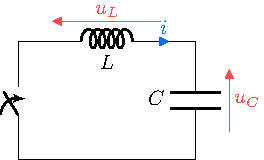
\includegraphics[width=.65\linewidth]{lc_descendant-intens}
    \end{center}
\end{defi}

\vspace*{-15pt}
\subsection{Équation différentielle du circuit}
\begin{tcbraster}[raster columns=2, raster equal height=rows]
    \begin{prop}[label=prop:eqdiffrc]{équation diff. RC}
        L'équation différentielle de la tension $u_C(t)$ aux bornes d'un
        condensateur dans un circuit LC en décharge est
        \[ \boxed{\dv[2]{u_C}{t} + \w_0{}^2u_C = 0}\]
        avec \fbox{$\w_0 = \frac{1}{\sqrt{LC}}$} la pulsation propre.
        \tcblower
        Les conditions initiales (continuité de $u_C$ aux bornes de $C$
        et de $i$ traversant $L$) sont
        \begin{empheq}[box=\fbox]{gather*}
            u_C(0^-) = u_C(0^+) = E\\
            i(0^-) = i(0^+) = 0
        \end{empheq}
    \end{prop}
    \begin{demo}[label=demo:eqdiffrc]{équation diff. RC}
        Avec la loi des mailles,
        $$u_L + u_C = 0$$
        Ensuite, \textbf{en convention récepteur} on a~:
        $\DS u_L = L \dv{i}{t}$ et $\DS i = C \dv{u_C}{t}$
        \begin{gather*}
            L \dv{i}{t} + u_C                                = 0
            \Leftrightarrow LC \dv[2]{u_C}{t} + u_C          = 0\\
            \Leftrightarrow \dv[2]{u_C}{t} + \frac{1}{LC}u_C = 0
        \end{gather*}

        D'où le résultat. $L$ assure $i(0^+) = 0$ et $C$ assure $u_C(0^+) = E$
        par continuité.
    \end{demo}
\end{tcbraster}

%\vspace*{-15pt}
\begin{rema}[label=rema:unité]{Unité de $\w_0$}
    On peut vérifier à cette étape que $\w_0$ est bien homogène à l'inverse d'un
    temps. Pour ça, deux manières~:

    \begin{remaside}
        \textbf{Par analyse dimensionnelle directe}. Sachant que $RC$ et $L/R$
        sont des temps (cf.\ chapitre précédent)~:
        \begin{align*}
            w_0{}^2 = \frac{1}{LC} =
                \frac{\textcolor{cornflowerblue}{R}}
                {\textcolor{cornflowerblue}{L}\textcolor{orange}{RC}}
                = \underbrace{\left[ \frac{L}{R}
                \right]^{-1}}_{\si{s^{-1}}}\times
                \underbrace{\left[ RC \right]^{-1}}_{\si{s^{-1}}}
        \end{align*}

        Et on a bien $\w_0{}^2$ en \si{s^{-2}}, et donc $\w_0$ en \si{s^{-1}},
        les radians n'ayant pas de dimension.

        \tcblower
        \textbf{Par analyse dimensionnelle indirecte}. En effet, l'équation
        différentielle est forcément une équation homogène. Aisi
        \begin{equation*}
            \left[ \dv[2]{u_C}{t} \right] =
                \frac{\left[u_C\right]}{\left[\dt\right]^2}\\
                                          = \frac{\si{V}}{\si{s^2}}
        \end{equation*}
        et l'autre terme doit avoir la même unité~:
        \begin{equation*}
            \left[ w_0{}^2u_C \right] = \left[ w_0 \right]^2\times \left[
            u_C \right]\\
                                      = \si{V.s^{-2}}
        \end{equation*}
        On en déduit que $\w_0{}^2$ est de dimension \si{s^{-2}}, d'où la
        dimension de $\w_0$.
    \end{remaside}
\end{rema}

\subsection{Résolution de l'équation différentielle et graphique}
\begin{tcbraster}[raster columns=2, raster equal height=rows]
    \begin{tcolorbox}[blankest, raster multicolumn=1, space to=\myspace]
        \begin{tcbraster}[raster columns=1]
            \begin{prop}[label=prop:ucsolu]{solution de l'équation
                différentielle RC}
                La solution de l'équation différentielle de la tension $u_C(t)$
                d'un circuit LC en décharge avec $u_C(0) = E$ et l'intensité en
                découlant sont
                \begin{empheq}[box=\fbox]{gather*}
                    u_C(t) = E\cos(\w_0t)\\
                    i(t) = -CE\w_0\sin(\w_0t)
                \end{empheq}
            \end{prop}
            \begin{NCexem}[width=\linewidth]{Graphique}
                \begin{center}
                    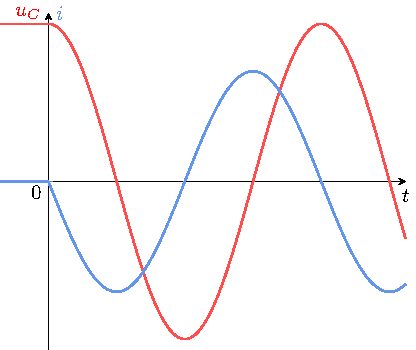
\includegraphics[width=\linewidth]{carac-lc_descendant-harmonique}
                \end{center}
            \end{NCexem}
        \end{tcbraster}
    \end{tcolorbox}
    \begin{demo}[label=demo:rcsolu]{solution RC série}
        L'équation étant déjà homogène, on écrit la forme générale~:
        \[u_C(t) = A\cos(\w_0 t) + B\cos(\w_0 t)\]

        Celle-ci est souvent plus pratique pour trouver les constantes
        d'intégration. On trouve $A$ avec la première condition initiale~:
        $u_C(0^+) = E$. En effet,
        \[u_C(0) = A\cos(0) + B\sin(0) = A\]
        donc $A=E$.\smallbreak

        On trouve $B$ avec la seconde condition initiale~: $i(0^+) = 0 = C
        \dv{u_C}{t}$. En effet,
        \begin{gather*}
            \dv{u_C}{t} = -A\w_0\sin(\w_0t) + B\w_0\cos(\w_0t)\\
            \Rightarrow \dv{u_C}{t} (0) = B\w_0
        \end{gather*}
        Donc $B = 0$ ($\w_0 \neq 0$). On obtient ensuite $i$ avec la relation
        courant-tension.
    \end{demo}
\end{tcbraster}

\subsection{Bilan énergétique}
\begin{tcbraster}[raster columns=2, raster equal height=rows]
    \begin{prop}[label=prop:lcenerg-décharge]{bilan d'énergie}
        L'énergie emmagasinée dans le circuit est
        \[\boxed{\Ec = \frac{1}{2}Cu_C{}^2 + \frac{1}{2}Li^2}\]
        Elle est conservée à chaque instant et résulte de l'échange périodique
        d'énergie entre le condensateur et la bobine.
    \end{prop}
    \begin{demo}[label=demo:rcenerg-charge]{bilan d'énergie}
        On fait un bilan de puissances avec la loi des mailles multipliée par $i$~:
        \begin{gather*}
            u_Ci + u_Li = 0\\
            \Leftrightarrow u_C\times C \dv{u_C}{t} + L \dv{i}{t}\times i = 0\\
            \Leftrightarrow \dv{}{t} \left( \frac{1}{2}Cu_C{}^2 + \frac{1}{2}Li^2 \right) = 0
        \end{gather*}
        On identifie l'intérieur de la parenthèse à l'énergie du système (car
        par définition $\Pc = \dv{\Ec}{t}$) pour avoir la propriété.
    \end{demo}
    \begin{impl}[label=impl]{vérification}
        On vérifie avec les expressions analytiques trouvées, sachant que
        $\w_0{}^2 = (LC)^{-2}$~:
        \begin{gather*}
            \frac{1}{2}Cu_C{}^2 = \frac{1}{2}CE^2\cos^2(\w_0t)\\
            \frac{1}{2}Li^2 =
            \frac{1}{2}\underbrace{LC^{2}\w_0{}^2}_{=C}E^2\sin^2(\w_0t)\\
            \Rightarrow \Ec = \frac{1}{2}CE^2 \left( \cos^2(\w_0t) +
            \sin^2(\w_0t) \right)
        \end{gather*}
        Soit
        \begin{equation*}
            \boxed{\Ec = \frac{1}{2}CE^2 = \text{cste}}
        \end{equation*}
    \end{impl}
    \begin{NCexem}[width=\linewidth]{Graphique}
        \begin{center}
            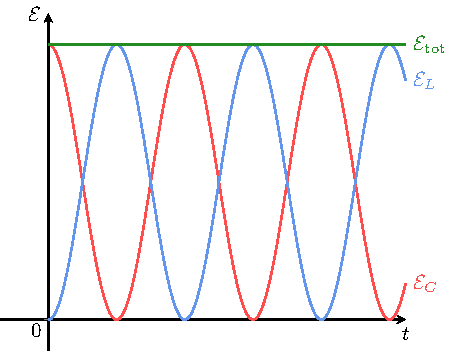
\includegraphics[width=\linewidth]{carac-lc_descendant-bilan}
        \end{center}
    \end{NCexem}
\end{tcbraster}

\begin{impo}[label=impo:amortissement]{résultat}

    On retrouve bien des oscillations de la tension aux bornes de $u_C$ comme
    dans l'approche expérimentale, avec une période $T_0 = \frac{2\pi}{\w_0} =
    2\pi\sqrt{LC}$ qui augmente avec $L$ et $C$. Cependant, \textbf{nous n'avons
    pas d'amortissement ici}~! En effet les composants utilisés ici sont idéaux,
    et conservent totalement l'énergie, il n'y a pas de raison d'en perdre. Il y
    a eu une simplification que l'on effectue souvent en mécanique~: \textbf{on
    a négligé les effets dissipatifs}. Regardons comment ça se traduit pour un
    exemple mécanique.

\end{impo}

\section{Exemple harmonique mécanique~: ressort horizontal libre}

\subsection{Introduction}

\begin{defi}[label=defi:ressortdef, sidebyside, righthand ratio=.5]{force de
    rappel d'un ressort}

    Soit le système masse-ressort horizontal représenté ci-contre. Le ressort se
    déforme sous l'effet d'une contrainte en stockant l'énergie donnée, qu'il
    libère en reprenant sa forme quand la contrainte s'arrête. On définit la
    force de rappel du ressort par~:

    \begin{equation*}
        \boxed{\vv*{F}{\rm rappel} = -k(\ell - \ell_0)\ux}
    \end{equation*}
    avec

    \begin{itemize}
        \item $k > 0$ la \textbf{constante de raideur} en $\si{N.m^{-1}}$
            ($[\vv{F}] = [k][\ell]$)~;
        \item $\ell_0$ sa \textbf{longueur à vide}~;
        \item $\ux$ un vecteur unitaire ($ \left\Vert \ux \right\Vert = 1$)
            dirigé selon l'axe $x$
    \end{itemize}

    \tcblower
    \begin{center}
        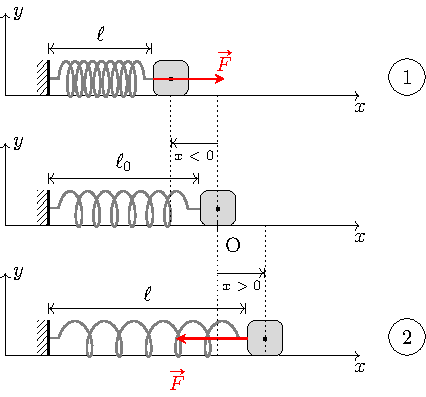
\includegraphics[width=\linewidth]{ressort_def}
    \end{center}

    Si $\ell > \ell_0$, on a bien une force dirigée selon $-\ux$, (situation
    \circled{2}), sinon dirigée selon $+\ux$.

\end{defi}

\subsection{Présentation}
\begin{defi}[label=def:ressortlibre, sidebyside, righthand ratio=.5]{situation
    initiale et bilan des forces}
    \begin{description}
        \item[Système] : point matériel $M$ de masse $m$ relié à un ressort
            horizontal \textbf{idéal et sans frottements}.
        \item[Référentiel] : $\Rc_{\rm sol} (O,x,y,t)$~;
    \end{description}

    \centers{\fbox{Soit $x = \ell - \ell_0$ la position de la masse}}\bigbreak

    \textbf{Conditions initiales}~:
    \begin{enumerate}[leftmargin=20pt]
        \item À $t=0$ la masse est à la position $x_0 > 0$~;
        \item À $t=0$ sa vitesse est $v_0 = 0$.
    \end{enumerate}

    \tcblower
    \begin{center}
        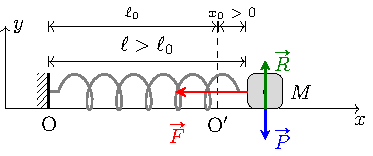
\includegraphics[width=\linewidth]{ressort_libre}
    \end{center}

    \textbf{Bilan des forces}~:
    \begin{enumerate}
        \item Poids $\Pf = -mg\uy$~;
        \item Réaction du support $\vv{R} = R\uy$~;
        \item Force de rappel du ressort $\Ff = -kx\ux$
    \end{enumerate}

\end{defi}

\subsection{Équation différentielle et solution}

\begin{tcbraster}[raster columns=2, raster equal height=rows]
    \begin{prop}[label=prop:eqdiffreslibre]{équation et solution}
        La position $x$ de la masse et la longueur $\ell$ du ressort sont régies
        par~:

        \begin{empheq}[box=\fbox]{gather*}
             \dv[2]{x}{t} + \w_0{}^2x = 0\\
             \Leftrightarrow \dv[2]{\ell}{t} + \w_0{}^2\ell = \w_0{}^2\ell_0
        \end{empheq}

        Avec $\w_0 = \DS \sqrt{\frac{k}{m}}$. $\ell_0$ est donc la longueur
        d'équilibre du système.
        \tcblower
        La position $x$ et la vitesse $v$ ont pour expression
        \begin{empheq}[box=\fbox]{gather*}
            x(t) = x_0\cos(\w_0t)\\
            v(t) = -x_0\w_0\sin(\w_0t)
        \end{empheq}
    \end{prop}
    \begin{demo}[label=demo:solreslibre]{équation différentielle}
        La deuxième loi de \textsc{Newton}, aussi appelée \textbf{principe
        fondamental de la dynamique} (PFD) donne~:
        \begin{gather*}
            m\af = \Pf + \vv{R} + \Ff\\
            \Leftrightarrow m\left(
                \begin{array}{c}
                    \dv[2]{x}{t}\\
                    0
                \end{array}
            \right)
            =
            \left(
                \begin{array}{c}
                    -kx\\
                    -mg + R
                \end{array}
            \right)
        \end{gather*}
        Sur l'axe $\ux$ on trouve bien $m \dv[2]{x}{t} + kx = 0$, d'où
        l'équation différentielle. La projection sur $\uy$ montre que la
        réaction du support compense le poids.
        \tcblower
        On a la même démonstration que précédemment.
    \end{demo}
\end{tcbraster}
\begin{rema}[label=rema:ressortlibre, sidebyside]{analogie LC-ressort}
    Alors qu'on partait d'un système \textit{a priori} totalement différent, on
    remarque que la physique des deux systèmes sont rigoureusement équivalentes
    puisque \textbf{régies par la même équation différentielle}. On observe une
    oscillation du ressort autour d'une position d'équilibre, ici $x=0
    \Leftrightarrow \ell = \ell_0$.
    \tcblower
    On peut donc associer $u_C$ à $x$ et $i$ à $v$, étant donné que pour un
    condensateur $i = C \dv{u_C}{t}$ et que $v = \dv{x}{t}$. Ainsi, \textbf{les
    échanges énergétiques sont les mêmes} entre l'énergie emmagasinée dans la
    déformation du ressort et l'énergie cinétique de la masse comme on va le
    voir juste après.
\end{rema}

\subsection{Bilan énergétique}

\begin{tcbraster}[raster columns=2, raster equal height=rows]
    \begin{defi}[label=def:emeca]{énergies potentielle élastique et mécanique}
        Le ressort emmagasine une énergie \textit{potentielle} lors de sa
        déformation, telle que
        \[\boxed{\Ec_{p\rm, el} = \frac{1}{2}k(\ell-\ell_0)^2 = \frac{1}{2}kx^2}\]
        On définit alors l'énergie mécanique totale $\Ec_m$ du système par
        \[\boxed{\Ec_m = \Ec_c + \Ec_p}\]
        avec, évidemment, $\Ec_c = \frac{1}{2}mv^2$.
    \end{defi}
    \begin{tcolorbox}[blankest, raster multicolumn=1, space to=\myspace]
        \begin{tcbraster}[raster columns=1]
            \begin{prop}[label=prop:emecacons]{conservation énergie}
                Dans le système masse-ressort horizontal sans frottements, l'énergie
                mécanique est conservée.
            \end{prop}
            \begin{demo}[label=demo:emecacons]{conservation énergie}
                À partir de l'équation différentielle on multiplie par $\dv{x}{t}$ et on
                utilise que $ff' = (\frac{1}{2}f^2)'$ pour $f$ une fonction~:
                \begin{gather*}
                    m \dv[2]{x}{t} \dv{x}{t} + kx \dv{x}{t} = 0\\
                    \Leftrightarrow \dv{}{t} \left( \frac{1}{2}m \left( \dv{x}{t} \right)^2 +
                    \frac{1}{2}kx^2 \right) = 0
                \end{gather*}
                On a bien $ \frac{1}{2}mv^2 + \frac{1}{2}kx^2 = \Ec_m$ conservé.
            \end{demo}
        \end{tcbraster}
    \end{tcolorbox}
    \begin{impl}[label=impl]{vérification}
        On vérifie avec les expressions analytiques trouvées, sachant que
        $\w_0{}^2 = \frac{k}{m}$~:
        \begin{gather*}
            \frac{1}{2}kx^2 = \frac{1}{2}kx_0{}^2\cos^2(\w_0t)\\
            \frac{1}{2}mv^2 =
            \frac{1}{2}\underbrace{m\w_0{}^2}_{=k}x_0{}^2\sin^2(\w_0t)\\
            \Rightarrow \Ec_m = \frac{1}{2}kx_0{}^2 \left( \cos^2(\w_0t) +
            \sin^2(\w_0t) \right)
        \end{gather*}
        Soit
        \begin{equation*}
            \boxed{\Ec_m = \frac{1}{2}kx_0{}^2 = \text{cste}}
        \end{equation*}
    \end{impl}
    \begin{NCexem}[width=\linewidth]{Graphique}
        \begin{center}
            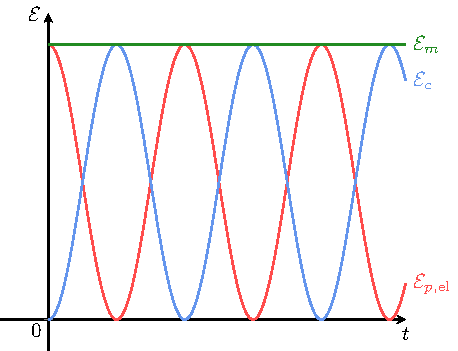
\includegraphics[width=\linewidth]{carac-ressort_libre-bilan}
        \end{center}
    \end{NCexem}
\end{tcbraster}

\vspace*{-20pt}
\subsection{Analyse correspondance}
\begin{NCexem}[width=\linewidth, sidebyside, righthand ratio=.4]{Visualisation}

    Il est utile d'observer la physique des systèmes oscillants non pas dans
    un espace (grandeur, temps) mais dans un espace \textbf{(grandeur,
    dérivée)}, qui permet plus rapidement de sonder son évolution. Par
    exemple, le ressort lâché à $x_0$ et $v_0=0$ voit sa position diminuer
    et sa vitesse augmenter (algébriquement) jusqu'à ce qu'il passe par sa
    position d'équilibre ($x=0$) avec une vitesse extrémale $v_{\min}$,
    avant de se comprimer en perdant de sa vitesse. Comme il n'y a
    \textbf{pas de perte dans cette étape}, elle se répète
    \textbf{symétriquement} en revenant à son point de départ.

    \tcblower
    \begin{center}
        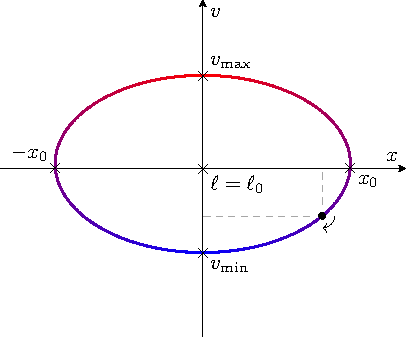
\includegraphics[width=\linewidth]{carac-ressort_libre-xy}
    \end{center}
\end{NCexem}

\begin{framed}
    En réalité, frottements existent, ou résistance existe~: amortissement.
\end{framed}

\section{Complément~: circuit LC montant}

\subsection{Présentation}

\subsection{Équation différentielle}

\subsection{Solution et représentation}

\subsection{Changement de variable~: de générale à homogène}

LC série montant. Équation différentielle avec $\w_0{}^2E$. $x = x-E$
fonctionne. ATTENTION~: CI différentes~! $u_C(t=0) = 0$ et $i(t=0) = 0$. $A =
-E$, $B=0$, $u_C = E - E\cos(\w_0t)$. Graphique.

\subsection{Intérêt oscillateur harmonique}

Le principal intérêt de l'observation régulière d'une oscillation est la mesure
du temps. Une excitation quelconque (comme un échelon) produit un phénomène se
reproduisant à intervalle régulier et fait alors apparaître un étalon
temporel. Ce principe est utilisé~:
\begin{itemize}
    \item dans les horloges mécaniques à balancier~: on exploite le mouvement
        régulier du pendule~;
    \item dans les horloges à ressort~: la période est liée au rapport de
        l'inertie et de la raideur du système~;
    \item dans les horloges électroniques~: un cristal de quartz dont la
        fréquence d'oscillation est précisément connue (en général une puissance
        de 2 en Hz)~;
    \item dans les horloges atomiques~: on utilise la régularité des
        oscillations des ondes électromagnétiques absorbées par un atome.
        L'actuelle définition de la seconde est basée sur le fonctionnement
        d'une horloge atomique.
\end{itemize}


\section{Introduction amorti}

\subsection{Équation différentielle}

\begin{prop}[label=prop:eqdiffoh]{équation différentielle}
    Équilibre $x_{\rm eq}$
    \[ \boxed{ \dv[2]{x}{t} + \frac{\w_0}{Q} \w_0{}^2x = \w_0{}^2x_{\rm eq}}\]
    Avec $\w_0$ la pulsation \textbf{propre}, et $Q$ facteur de qualité.
\end{prop}

\subsection{Évolutions en régime libre, exemple RLC}

En réalité, nous observons que les oscillations dans le circuit s’atténuent. Plus quantitativement :

\begin{itemize}
    \item Lorsque la résistance est petite : on observe plusieurs oscillations.
        Nous avons câblé un circuit avec $L = \SI{43}{mH}$ et $C = \SI{20}{nF}$.
        On observe une série d’oscillations à la période $T = \SI{186}{\micro
        s}$. On observe environ 25 oscillations lorsque $R \approx
        \SI{60}{\ohm}$ (résistance interne du GBF + de la bobine), 9
        oscillations lorsque $R \approx \SI{180}{\ohm}$, 3 oscillations lorsque
        $R \approx \SI{780}{\ohm}$.

    \item Lorsque la résistance est plus grande : les oscillations
        disparaissent. Lorsque $R \approx \SI{2,8}{k\ohm}$, on observe un régime
        transitoire dont la durée est d’environ $\SI{250}{\micro s}$ (à 95\%).
        Lorsque $R \approx \SI{10,8}{k\ohm}$, on observe un régime transitoire
        plus long, d’environ \SI{900}{\micro s}.

\end{itemize}

\section{Oscillateur amorti électrique~: circuit RLC série libre}

\subsection{Présentation}

\subsection{Bilan énergétique}

\subsection{Équation différentielle}

\subsection{Solutions}
\subsubsection{Conditions initiales}
\subsubsection{Équation caractéristique}
\subsubsection{Cas $\D < 0$~: régime pseudo-périodique}
\subsubsection{Cas $\D = 0$~: régime critique}
\subsubsection{Cas $\D > 0$~: régime apériodique}


\end{document}
